\documentclass{article}
\usepackage[utf8]{inputenc}
\usepackage{graphicx}
\usepackage{amssymb}
\graphicspath{{Images/}}
\usepackage{chngcntr}
\usepackage{cancel}
\counterwithin{equation}{section}

\title{Problem Set 2 (Astrophysics)}
\author{Michael Nameika}
\date{February 4 2022}

\begin{document}

\maketitle

\section{}
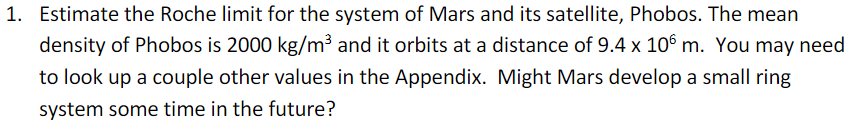
\includegraphics[scale = 0.8]{probset2prob1.PNG}


From the problem above, we have 
\begin{equation}
    \rho_{Phobos} = 2000 \frac{kg}{m^3}
\end{equation}
and
\begin{equation}
    r_{Phobos-Mars} = 9.4 \times 10^6 \:m
\end{equation}
From the astronomical data in the Physics Hypertextbook we have the following for the radius and mass of Mars:
\begin{equation}
    R_{Mars} = 3389.5 \: km
\end{equation}
\begin{equation}
    M_{Mars} = 6.39 \times 10^{23} \: kg
\end{equation}
Now, we can find the density of Mars using $\rho = \frac{M}{V}$,
  \[  \rho_{Mars} = \frac{6.39 \times 10^{23} \: kg}{\frac{4}{3}\pi(3.39 \times 10^6 \:m)^3}\]
\begin{equation}
    = 3916 \: \frac{kg}{m^3}
\end{equation}
Now, using the following equation to find the Roche limit of the Mars-Phobos system,
\begin{equation}
    r_{Roche} = 2.44*(\frac{\rho_{Mars}}{\rho_{Phobos}})^{1/3}R_{Mars}
\end{equation}
Plugging in (1.1), (1.3), and (1.5) into the above equation, we get
\[ = 2.44*(\frac{3916 \: \frac{\cancel{kg}}{\cancel{m^3}}}{2000 \: \frac{\cancel{kg}}{\cancel{m^3}}})*^{1/3}3.390\times 10^6 \: m\]
\begin{equation}
    \approx 1.035\times 10^7 \: m
\end{equation}
And we can see that (1.2) is less than (1.7), so Phobos is indeed within the Roche limit of Mars! If Phobos is held together by self gravitational forces, then it may be the case in the "near" future that Phobos could turn into a ring around Mars. However, if Phobos is instead held together by electrical forces, then Phobos is probably fine.







\section{}


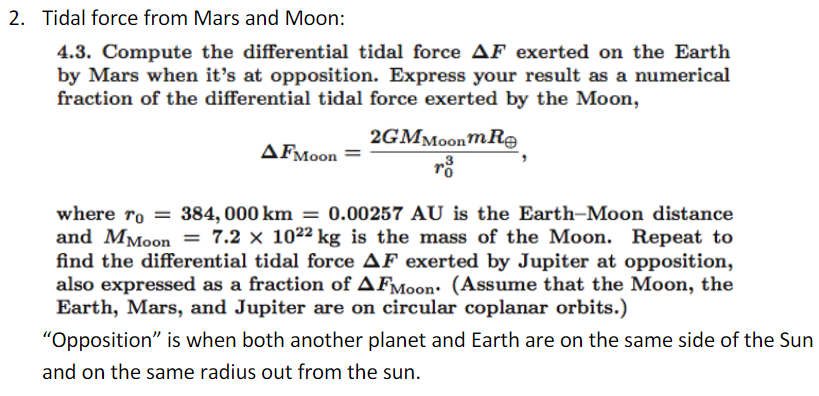
\includegraphics[scale = 0.8]{probset2prob2.PNG}
We can find the tidal force on the Earth from mars by the following:
\begin{equation}
    \Delta F_{Mars} = \frac{2GM_{Mars}mR_{Earth}}{r_1^3}
\end{equation}
Where $r_1$ is the distance between Earth and Mars when Mars is at opposition. Using that the average distance from the Sun to Mars is approximately $1.5 \: AU$, we can find $r_1$ by



\begin{equation}
    r_1 = 1.5 \: AU - 1 \: AU = 0.5 \: AU
\end{equation}

Then the ratio between $\Delta F_{Mars}$ and $\Delta F_{Moon}$:
\[\frac{\Delta F_{Mars}}{\Delta F_{Moon}} = \frac{\frac{\cancel{2G}M_{Mars}\cancel{m}\cancel{R_{Earth}}}{r_0^3}}{\frac{\cancel{2G}M_{Moon}\cancel{m}\cancel{R_{Earth}}}{r_1^3}}\]
\[ = \frac{M_{Mars}r_0^3}{M_{Moon}r_1^3}\]
\[ = \frac{6.390 \times 10^{23} \: \cancel{kg} * (0.00257 \:\cancel{AU})^3 }{7.200 \times 10^{22} \: \cancel{kg} * (0.5 \: \cancel{AU})^3}\]
\begin{equation}
    \approx 1.205 \times 10^{-6}
\end{equation}
That is, (2.3) tells us that the tidal force on Earth by Mars at opposition is roughly 1 million times weaker than that of the Moon.
\newline\newline
We also wish to find the ratio between the tidal force of Jupiter at opposition with that of the Moon.
Similar to the equation for the tidal force of Mars on the Earth, the tidal force on the Earth by Jupiter is given by
\begin{equation}
    \Delta F_{Jupiter} = \frac{2GM_{Jupiter}mR_{Earth}}{r_2^3}
\end{equation}
And using that the average distance between the Sun and Jupiter is approximately $5.2 \: AU$. So we can find the distance between the Earth and Jupiter by 
$r_2 = 5.2 \: AU - 1 \: AU = 4.2 $
Then the ratio between $\Delta F_{Jupiter}$ and $\Delta F_{Moon}$:
\[\frac{\Delta F_{Jupiter}}{\Delta F_{Moon}} = \frac{\frac{\cancel{2G}M_{Jupiter}\cancel{m}\cancel{R_{Earth}}}{r_2^3}}{\frac{\cancel{2G}M_{Moon}\cancel{m}\cancel{R_{Earth}}}{r_0^3}}\]
\[ = \frac{M_{Jupiter}r_0^3}{M_{Moon}r_2^3}\]
\[ = \frac{1.900 \times 10^{27} \: \cancel{kg} * (0.00257 \: \cancel{AU})^3}{7.200 \times 10^{22} \: \cancel{kg} * (4.2 \: \cancel{AU})^3}\]
\begin{equation}
    \approx 6.046 \times 10^{-6}
\end{equation}
Thus, the tidal force of Jupiter on the Earth is roughly 160,000 times weaker than that of the Moon on the Earth. Notice that Jupiter's tidal force is about 5x stronger than that of Mars on Earth!

\section{}
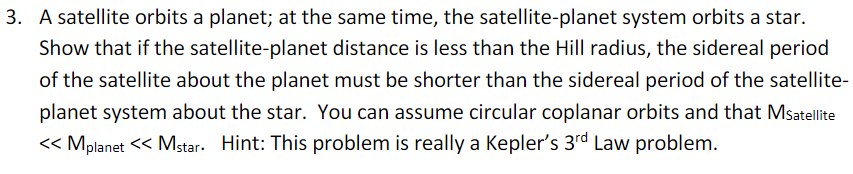
\includegraphics[scale = 0.8]{probset2prob3.PNG}
Recall Kepler's third law:
\begin{equation}
    P^2 = \frac{4 \pi^2}{G(m_1 + m_2)}a^3
\end{equation}
And recall the formula for Hill's radius:
\begin{equation}
    r_{Hill} \approx a(\frac{m}{2M})^{1/3}
\end{equation}
Consider some planet orbiting a star with a satellite such that $M_{Satellite} << M_{Planet} << M_{Star}$ such that the moon orbits within the planet's Hill radius. We wish to show that the sidereal period of the satellite about this planet is shorter than the sidereal period of the satellite-planet system.
\newline\newline
Proof: By equation (3.1), we have that the sidereal period of the planet-satellite system is given by 
\begin{equation}
    P_{P-Star}^2 = \frac{4 \pi^2}{G(M_{Star} + M_{Planet})}a_{P-Star}^3
\end{equation}
Now, by equation (3.2), the Hill radius of the planet-satellite system is given by
\begin{equation}
    r_{H, P-Sat} \approx a_{P-Sat}(\frac{M_{Satellite}}{2M_{Planet}})^{1/3}
\end{equation}
\[P_{P-Sat} < P_{P-Star}\]

Well, 
\[P_{P-Sat}^2 = \frac{4 \pi^2}{G(M_{Planet}+M_{Satellite})}a_{P-Sat}^3\]
\begin{equation}
    < \frac{4 \pi^2}{G(M_{Planet}+M_{Satellite})}a_{P-Star}^3(\frac{M_Planet}{M_Star})
\end{equation}
Since
\[M_{Satellite} << M_{Planet}\]
We can make the approximation
\begin{equation}
    \frac{4 \pi^2}{G(M_{Planet} + M_{Satellite})} \approx \frac{4 \pi^2}{GM_{Planet}}
\end{equation}
Substituting (3.6) into (3.5), we have the following:
\[P_{P-Sat}^2 < \frac{4 \pi^2}{G\cancel{M_{Planet}}} * a_{P-Star}^3*(\frac{\cancel{M_{Planet}}}{2M_{Star}})\]
\[= \frac{4 \pi^2}{2GM_{Star}}*a_{P-Star}^3\]
\[ = (\frac{1}{2})P_{P-Star}^2 \]
So we have
\[P_{P-Sat}^2 < \frac{1}{2}P_{P-Star}^2\]
\[P_{P-Sat} < \frac{1}{\sqrt{2}}P_{P-Star}\]
\[ < P_{P-Star}\]
And by transitivity, we finally have
\begin{equation}
    P_{P-Sat} < P_{P-Star}
\end{equation}
Thus, by (3.7), we have that the sidereal period of the satellite around the planet is less than the sidereal period of the planet-satellite system, as was desired.
\begin{flushright}
    $\square$
\end{flushright}


\section{}
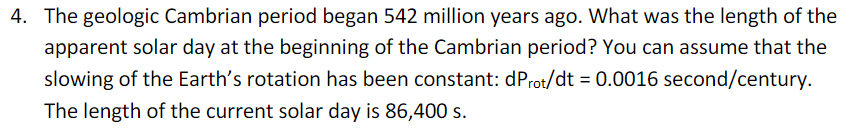
\includegraphics[scale = 0.8]{probset2prob4.PNG}

We are given that 
\begin{equation}
    \frac{dP_{rot}}{dt} = -0.0016 \: \frac{seconds}{century}
\end{equation}
And that the current solar day is
\begin{equation}
    t_{Today} = 86440 \: seconds
\end{equation}
To find how long a solar day was at the beginning of the Cambrian period, we simply need to find how many seconds Earth's rotation has slowed down in that period from equation (4.1), and add that time to (4.2).
\newline
The total time a day has slowed down by since the begging of the Cambrian is given by
\[t_{Cambrian} = t_{Solar} - \frac{dP_{rot}}{dt}\Delta t\]
where $\Delta t$ is the time since the Cambrian period, in centuries.
Well,
\[t_{Cambrian} = 86440 \: seconds + (-0.0016 \frac{seconds}{\cancel{century}})*(5.420\times 10^6 \: \cancel{centuries})\]
\begin{equation}
    t_{Cambrian} = 77768 \: seconds
\end{equation}
By (4.3) above, we can see that a Cambrian day was about 8600 seconds shorter than a current day, or about 2.5 hours shorter.

\section{}
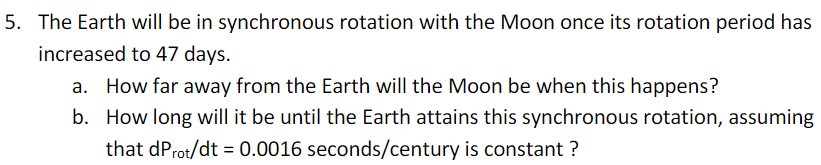
\includegraphics[scale = 0.8]{probset2prob5.PNG}
a) Recall Kepler's third law:
\begin{equation}
    P^2 = \frac{4 \pi^2}{G(M_1 + M_2)}a^3
\end{equation}
Solving for a, we get 
\begin{equation}
    a = (\frac{P^2G(M_1+M_2)}{4 \pi^2})^{1/3}
\end{equation}
Now, using $M_1 = M_{Earth} = 5.974 \times 10^{24} \: kg$ and $M_2 = M_{Moon} = 7.200 \times 10^{22} \: kg$, and the fact that $47 \: days = 4.061 \times 10^6 \: seconds$, and plugging this into equation (5.2), we find

    \[a_{Earth-Moon} = (\frac{(4.061 \times 10^{24} \: \cancel{s})^2 * (6.674 \times 10^{-11} \:m^3\cancel{kg^{-1}}\cancel{s^{-2}})*(5.974 \times 10^{24} \: \cancel{kg} + 7.200 \times 10^{22} \: \cancel{kg})}{4 \pi^2})^{1/3} \]
\[ = 5.524 \times 10^5 \: km\]
Compare this to the current distance of 
\[3.844 \times 10^5 \: km\]
b) Since the current length of an Earth day is, well, one day, we wish to find how long it will take for the Earth's rotation to slow down by 46 days. Well, we can find how long this will take by dividing 46 days by equation (4.1).
Before we do this, let us covert from days to seconds:
\[46 \: days = 3.974 \times 10^6 \: s\]
And dividing this by (4.1), we get
\[\Delta t = \frac{3.974 \times 10^6 \: \cancel{s} }{0.0016 \: \frac{\cancel{s}}{century}}\]
\[ = 2.484 \times 10^9 \: centuries\]
\[ = 2.484 \times 10^{11} \: years\]
So after about 248,400,000,000 years, the Earth's rotation will match the Moon's rotation rate.

\end{document}